\documentclass[12pt,letterpaper]{article}
\usepackage{graphicx}
\usepackage{geometry}
\usepackage{setspace}
\usepackage{anyfontsize}
\usepackage{parskip}
\usepackage{indentfirst}
\usepackage{amsmath}
\usepackage{cite}
\usepackage{listings}
\usepackage{color}
\usepackage{textcomp}
\usepackage{float}
\usepackage[utf8]{inputenc}
\usepackage{natbib}
\usepackage{subcaption}
\usepackage{enumitem}

\geometry{letterpaper, portrait, margin=1in}
\doublespace
\title{The Representation, Generation and Industry Application of B\'ezier Curves}
\author{Tynan Purdy}
\date{\vspace{-5ex}}
\graphicspath{{../Diagrams/}}

\definecolor{codegreen}{rgb}{0,0.6,0}
\definecolor{codegray}{rgb}{0.5,0.5,0.5}
\definecolor{codepurple}{rgb}{0.58,0,0.82}
\definecolor{backcolor}{rgb}{0.95,0.95,0.92}

\lstdefinestyle{scheme}{
    backgroundcolor=\color{backcolor},
    commentstyle=\color{codegreen},
    keywordstyle=\color{blue},
    numberstyle=\tiny\color{codegray},
    stringstyle=\color{codepurple},
    basicstyle=\footnotesize\ttfamily,
    breakatwhitespace=false,
    breaklines=true,
    captionpos=t,
    keepspaces=true,
    numbers=left,
    numbersep=5pt,
    showspaces=false,
    showstringspaces=false,
    showtabs=false,
    tabsize=2
}

\lstset{style=scheme}

\begin{document}
\large
\parindent=0.5in
{\fontsize{12}{14.4}
	{\singlespace
	    \pagenumbering{gobble}
	    \maketitle
	    \begin{center}
	    \vspace{4mm}
	    002129-0002 \\
	    \vspace{4mm}
	    IB Extended Essay \\
	    \vspace{4mm}
	    Mathematics \\
	    \vspace{4mm}
	    February 2019 \\
	    \vspace{4mm}
	    Words: 2592 \\
	\end{center}
	}
}	

\newpage
\pagenumbering{arabic}
%TC:break Abstract
\begin{abstract}
Curves are everywhere; in architecture, in objects, and in books. At some point, many of those curves existed on a computer. Graphic designs, 3D models of products, paper documents, so much of our carpentered world is rendered on a computer before it ever sees the third dimension. Computer-Aided Design (CAD) programs have taken over the manufacturing industry with versatile and extensive software packages that simulate any physical object right on the computer. Graphic design programs are at the source of every print and digital display. But these computer programs must be able to produce curved lines and surfaces in a computationally efficient way, or else producing all the curves used every day would bring computer hardware to its knees. A French automotive engineer by the name of Pierre B\'ezier implemented an efficient and easily adjustable method of digital curve rendering called the B\'ezier curve. His method of curve drawing has made its way into countless digital mediums, including 3D and 2D design software, digital typefaces, and more.

Words: 169

\end{abstract}
%TC:break _main_

\newpage
\tableofcontents

\newpage
\section{Introduction}
B\'ezier curves, a mathematical process for drawing curves, has found its way into the lifeblood of modern communication, digital graphics, and text. Every screen in the world is almost constantly using B\'ezier curves to draw whatever it is displaying. Most technology users do not know what B\'ezier curves are, despite looking at them every day for hours on end.  The lines of text on this very page were drawn using B\'ezier curves. The art on billboards was rendered with B\'ezier curves before they were ever printed. The ability to render virtual text characters instantaneously has contributed to the content boom of the internet. The following pages will describe what B\'ezier curves are, where they came from, and exactly how they are used to deliver words and shapes to the world.

The mathematics behind B\'ezier curves existed for decades before computers were invented. It was the French automotive engineer, Pierre B\'ezier (1910-1999), who popularized the method for digital curve and surface drawing. B\'ezier was a mathematician and head of design at Renault, a Paris based automaker \citep{handbook}. Before the origin of these special curves is discussed, it must be understood why curves are important and so difficult to procure digitally.
Curves have been used in mechanical design for hundreds of years, and for good reason. They give a smooth, attractive form that is not only more inviting to the touch than a sharp edge, but also lends itself toward aerodynamics. Curves are perfect for effortlessly passing through fluids such as air and water, as demonstrated in Figure \ref{fig:fluid}.

\begin{figure}[H]
    \begin{center}
    \caption{Fluid is redirected harshly around a cornered object relative to a rounded object.}
    \label{fig:fluid}
    \begin{subfigure}[b]{.4\linewidth}
        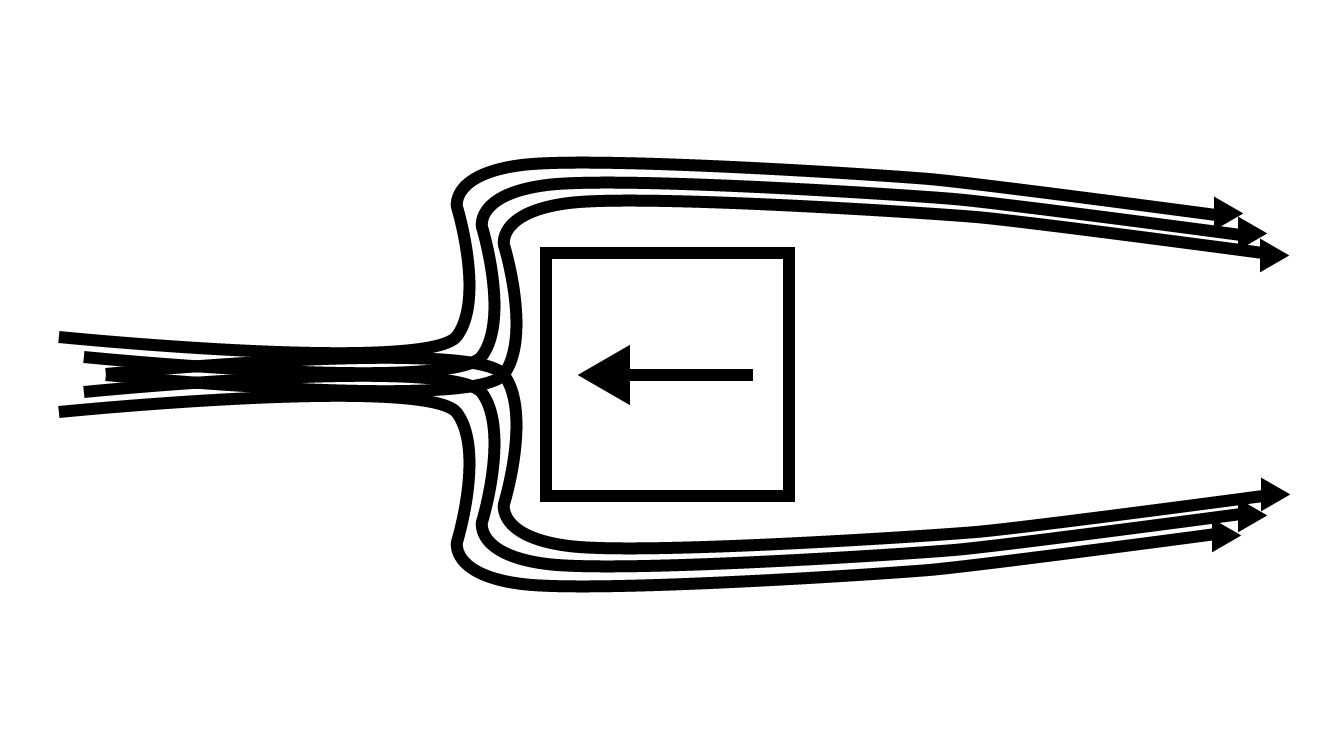
\includegraphics[width=\linewidth]{aero-square}
        \caption{Cornered object}
    \end{subfigure}
    \begin{subfigure}[b]{.4\linewidth}
        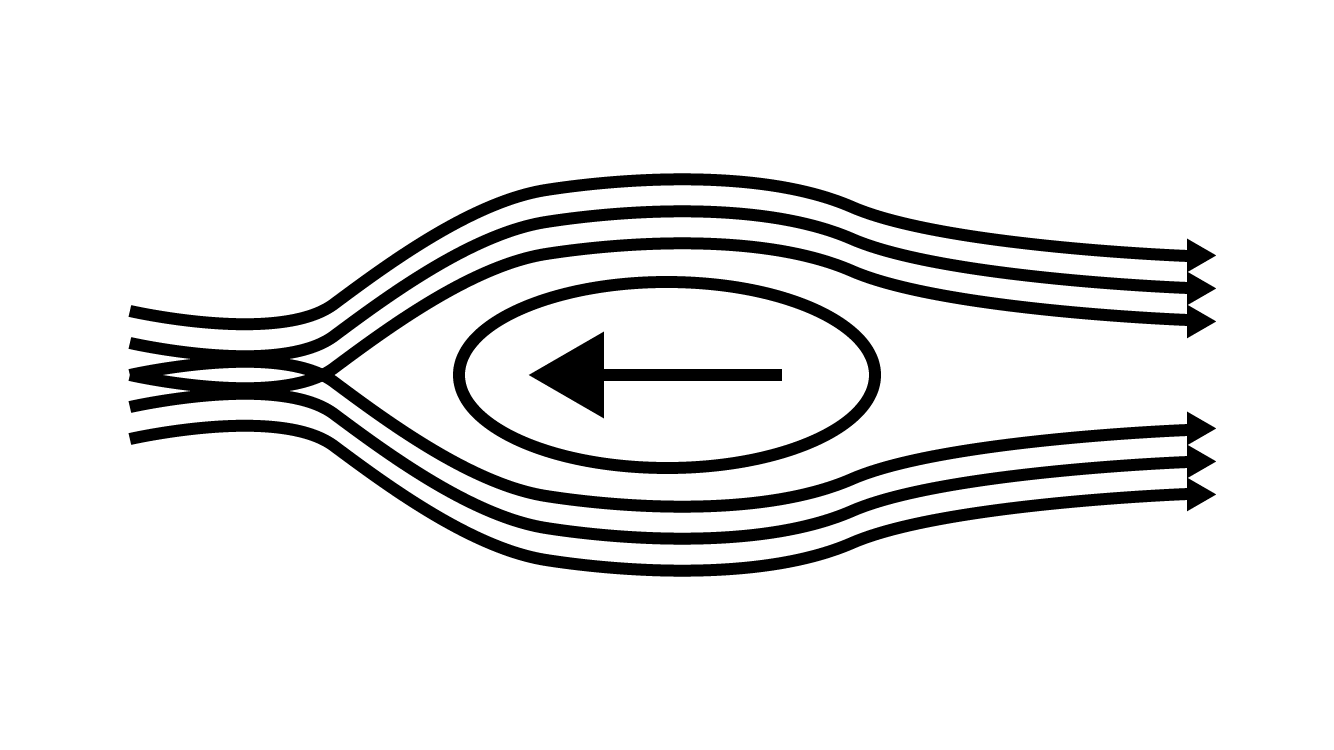
\includegraphics[width=\linewidth]{aero-curve}
        \caption{Rounded object}
    \end{subfigure}
\end{center}
\end{figure}

Unsurprisingly, aerodynamics in air and water accounts for the primary uses of curved surfaces both in ancient Rome and today. Consider the cars seen on the road today. Even an astute observer would have a hard time finding a perfectly flat surface or hard corner anywhere on a vehicle. Geometric patterns are so popular in the 21\textsuperscript{st} century, yet they have not made their way to cars. Curves are so energy efficient compared to straight lines and corners that there is no compelling reason to abandon them. 

Curves are also much safer than square edges and corners. Even objects that appear to have square corners often have a small fillet to smooth them out and avoid potential accidental cuts or scratches. The safe properties of curves arise from the same traits as its aerodynamic properties. An angled edge is more able to split open a solid that a curved edge (hence why knives must be sharp to function properly). The concern of safety against hard edges is addressed extensively in the manufacturing space. A wide variety of tools exists purely to reduce sharp edges to a smooth and safe curve.

Curved edges and surfaces clearly have their benefits. As discussed, there are ways to add curves to a cornered object, but it would be better to include curves in the original design. With manually operated tools, creating a curve is not particularly difficult. The human brain can visualize a shape and instruct the hands to use tools to make any shape or surface imaginable that the tool is capable of creating. Handcrafted wood objects can be curved with a chisel and some sanding. In the car manufacturing industry, most auto bodies are modeled at full scale in clay during the design phase. Handcrafting is sufficient for many purposes, but when the end goal of a design is to mass-produce it, at some point the shape of the object must be described by a computer. Manually operated tools are time consuming and labor intensive to make thousands of identical parts for mass production, which is not feasible for large scale manufacturing. Computer numerical control (CNC) tools have solved the mass production issue by allowing tools to be programmed to execute precise operations precisely and repeatably. CNC tools require far less attention from a human operator and produce consistent machining, perfect for mass production. The catch is, since the machine is computer controlled, the computer must be able to describe the cuts it is supposed to make, which means they must be described mathematically. Pierre B\'ezier was one of the first engineers to address the need for digital representation of physical parts, and so began development of the B\'ezier curve for Renault, his French automotive employer. B\'ezier was not the first, nor the only engineer to work on a mathematical curve algorithm for computers, but his was the widely adopted method. The famous De Casteljau’s algorithm was developed for Citroën, a competing auto company in Paris. His algorithm was kept secret for years after its development in the ‘60s \citep{handbook}, but later became the dominant method of producing B\'ezier curves on a computer. 

\section{B\'ezier Curves}

A B\'ezier curve is comprised of two major components: control points and Bernstein polynomials. The final curve is produced by a summation of Bernstein polynomials with the control point coordinate as a coefficient of each polynomial term. The Bernstein portion of the formula will be discussed before the complete De Casteljau algorithm.

\subsection{Bernstein Polynomials}
Bernstein polynomials are the expression that represent B\'ezier curves digitally. Before understanding B\'ezier curves mathematically, Bernstein polynomials must be defined. Bernstein functions are a method of approximating more complex polynomials. Linear polynomial terms are defined by Equation \ref{eq:bern}. Coefficients for each of the linear terms are given by the binomial coefficient formula (Equation \ref{eq:berncoeff}).

\begin{singlespace}
\begin{equation}
    \label{eq:bern}
    B_{n,i}(t) = \binom{n}{i} t^i (1-t)^{n-i} \qquad i=0,...,n
\end{equation}
\begin{small}
		\begin{itemize}[label=]
    	\item $n$: degree of the Bernstein function
    	\item $i$: iteration, or term
		\end{itemize}
\end{small}
\begin{equation}
    \label{eq:berncoeff}
    \binom{n}{i} = \prod_{i=1}^{n} \frac{n+1-i}{i}
\end{equation}
\end{singlespace}

Like any function, a Bernstein function of the degree $n$ will have $n+1$ many terms. The graphs below show the value of each individual term from $t=0$ to $t=1$ given different orders of the Bernstein function. 

\begin{figure}[H]
    \begin{center}
        \caption{Bernstein basis function graphs (Listing \ref{lst:bern})}
        \begin{subfigure}[b]{.3\linewidth}
            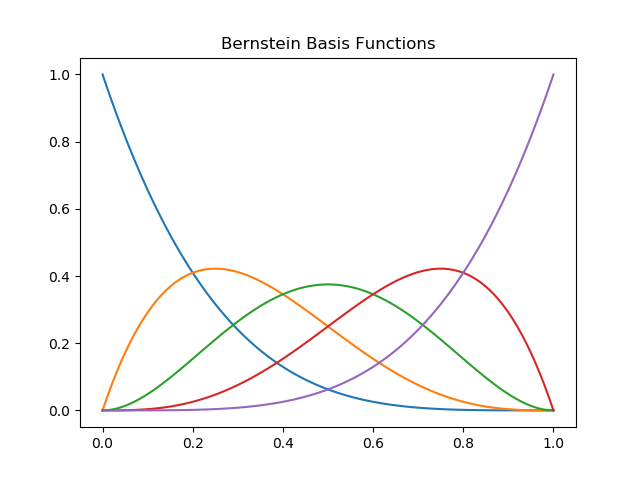
\includegraphics[width=\linewidth]{bern5}
            \caption{$n=4$}
        \end{subfigure}
        \begin{subfigure}[b]{.3\linewidth}
            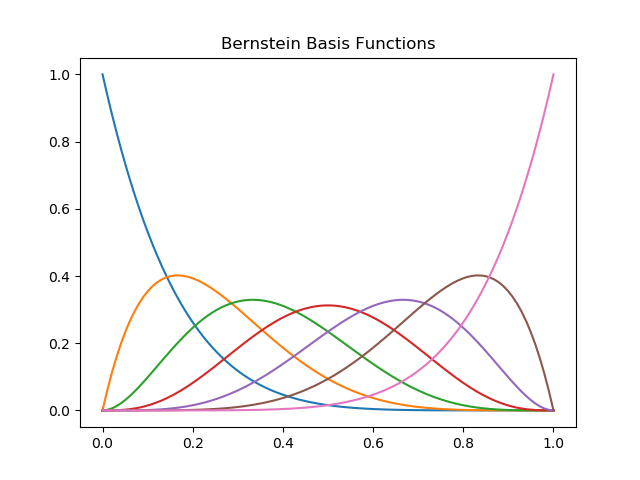
\includegraphics[width=\linewidth]{bern7}
            \caption{$n=6$}
        \end{subfigure}
        \begin{subfigure}[b]{.3\linewidth}
            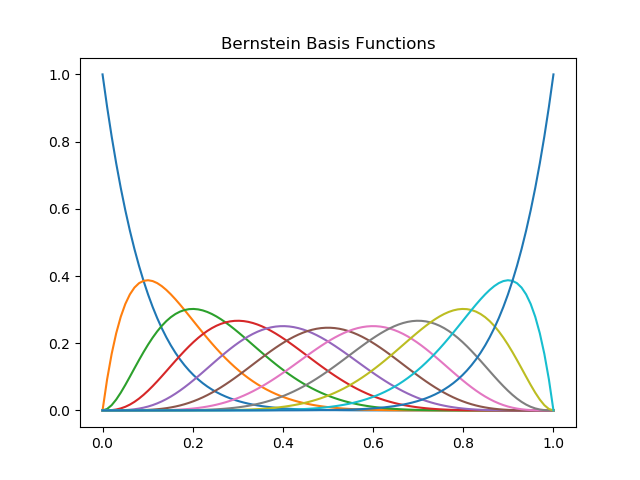
\includegraphics[width=\linewidth]{bern11}
            \caption{$n=10$}
        \end{subfigure}
    \end{center}
\end{figure}

The summation of the terms in a Bernstein polynomial is always equal to 1. Bernstein polynomials are used to approximate more complicated curved functions. Because the Bernstein function can create any shaped curve, it is well suited for this use case. 

\subsection{Parametric B\'ezier Curves}
A B\'ezier curve is a linear combination of Bernstein polynomials, each with coefficients corresponding to the coordinates of control points $P_i$. These control points are not necessarily intersected by the curve but they do determine its shape.

\begin{equation}
	\label{eq:decasteljau}
	F_{n}(t) = \sum_{i=0}^{n} P_{i} B_{n,i}(t)
\end{equation}

Because the algorithm in Equation \ref{eq:decasteljau} allows for any degree $n$ of B\'ezier curve, with any number of control points, Listing \ref{lst:bezier} was able be used to generate all of the B\'ezier curve figures in this section. With fewer than 50 lines of python code, any B\'ezier curve can be calculated and graphed. 

\begin{figure}[H]
    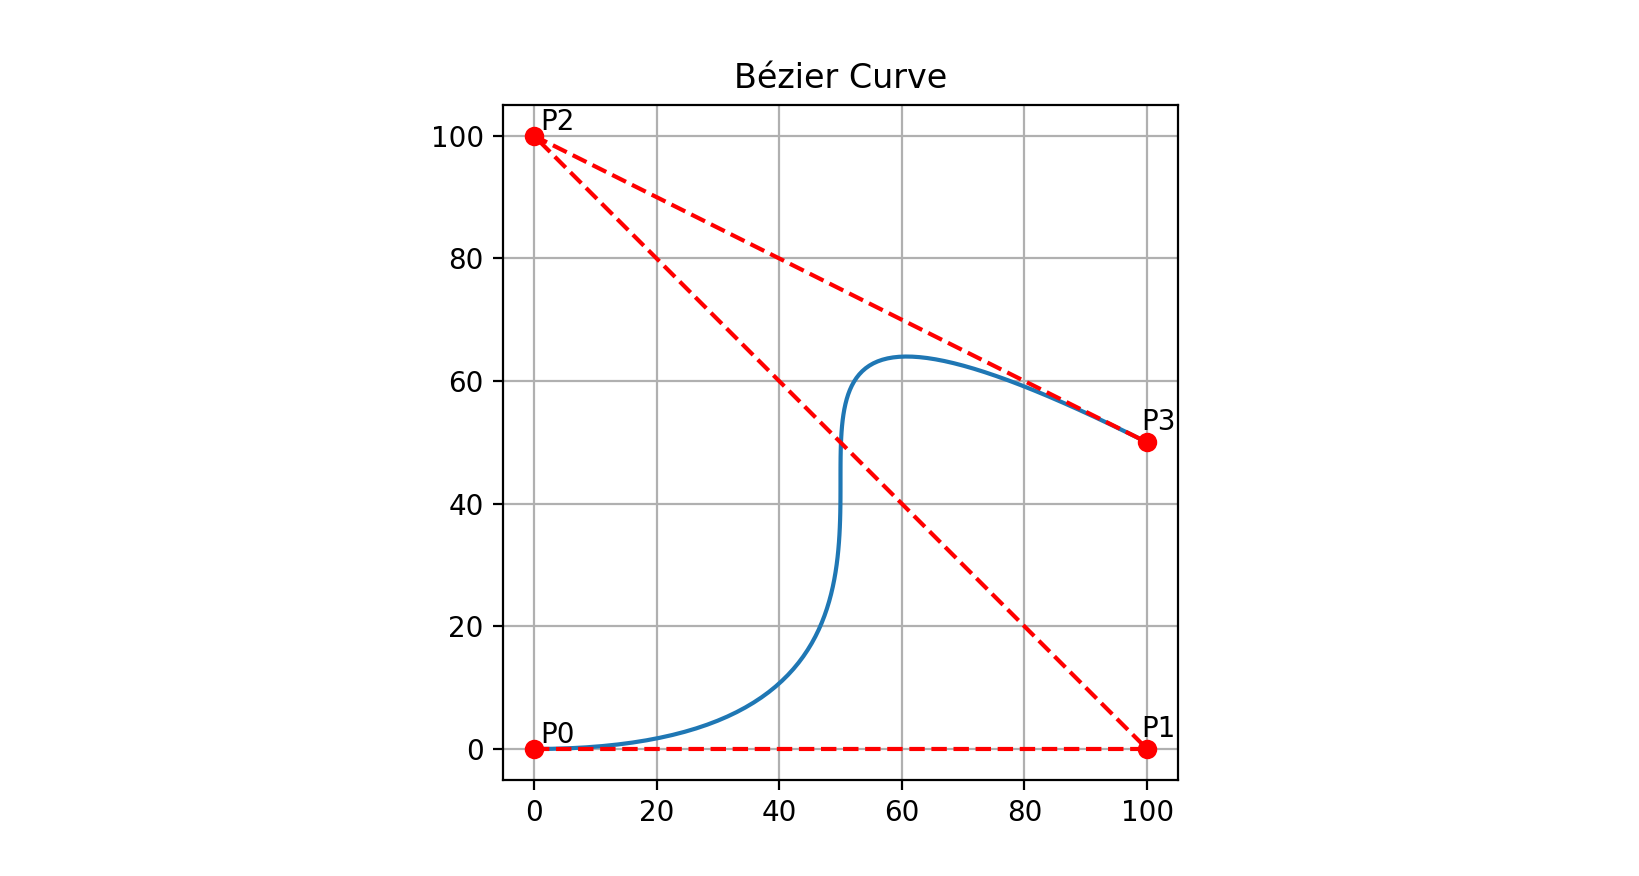
\includegraphics[width=15cm]{Figure_1}
    \centering
    \caption{B\'ezier curve with 4 control points.}
    \label{fig:demo}
\end{figure}

Consider Figure \ref{fig:demo}, a curve with four control points: $P_0, P_1, P_2,$ and $P_3$. $P_0$ and $P_3$ are the endpoints of the curve, so they will be intersected by the curve. $P_1$ and $P_2$ will not be intersected by the curve. They do \lq pull\rq \, the curve in their direction. Placing $P_1$ closer to a line between $P_0$ and $P_3$ will reduce the bend towards $P_1$.

\begin{figure}[H]
    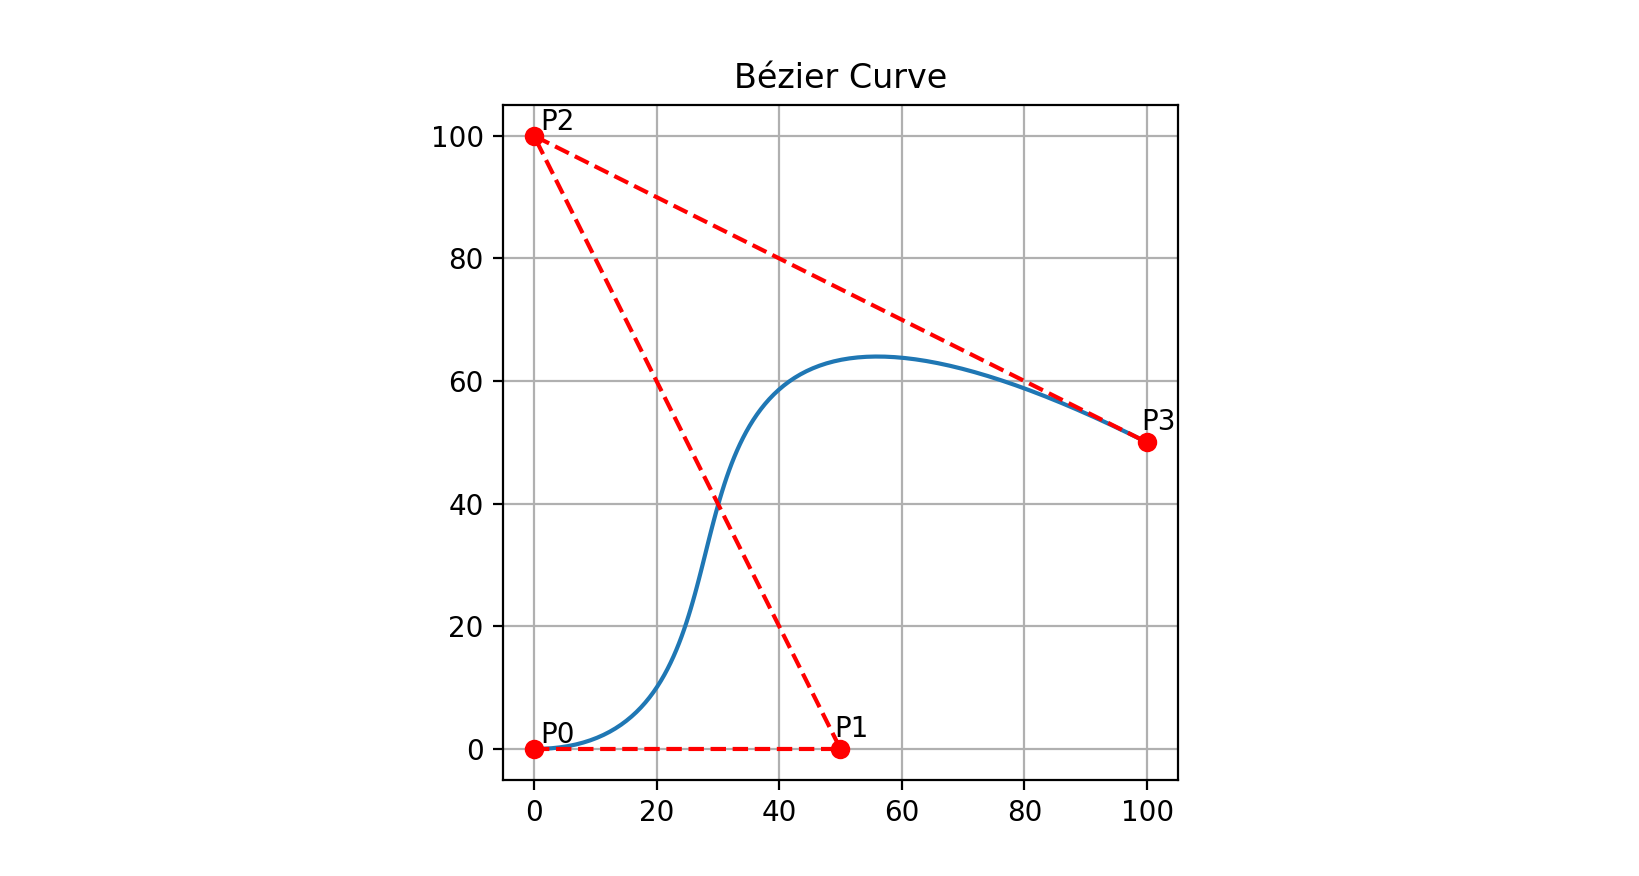
\includegraphics[width=15cm]{Figure_2}
    \centering
    \caption{Demonstration of how control points influence the curve. The closer the control points are to forming a line, the less curvature.}
    \label{fig:demo2}
\end{figure}

The behavior of the curve in relation to its control points comes from the properties of the equation that defines the curve. B\'ezier curves are defined by a parametric combination of Bernstein polynomials. While traditional graphed functions use an $x$-coordinate to solve for a $y$-coordinate, a parametric defines $x$ and $y$ individually as functions of time, $t$. 
Take Equation \ref{eq:para1} below. The parametric equation uses the parameter $t$ and two control points, $P_0$ and $P_1$. The equation is solved given $t$ from 0 to 1. At $t=0$, the result is equal to $P_0$, and at $t=1$ it is equal to $P_1$.

\begin{equation}
    \label{eq:para1}
    F(t) = P_0 + t(P_1 - P_0)
\end{equation}

In order to graph Equation \ref{eq:para1} as a linear B\'ezier curve (ignore the `linear curve' paradox, it works the same way), two control points must be designated, for instance $P_0(1, 1)$ and $P_1(2, 3)$. Then, the coordinates will be substituted into the parametric equation for $x$ and $y$.

$$x(t) = 1 + t(2-1)$$
$$y(t) = 1 + t(3-1)$$

Evaluating $x(t)$ and $y(t)$ from 0 to 1 produces coordinate points on the \lq curve\rq \, shown in Figure \ref{fig:bez2}. 

\begin{figure}[H]
    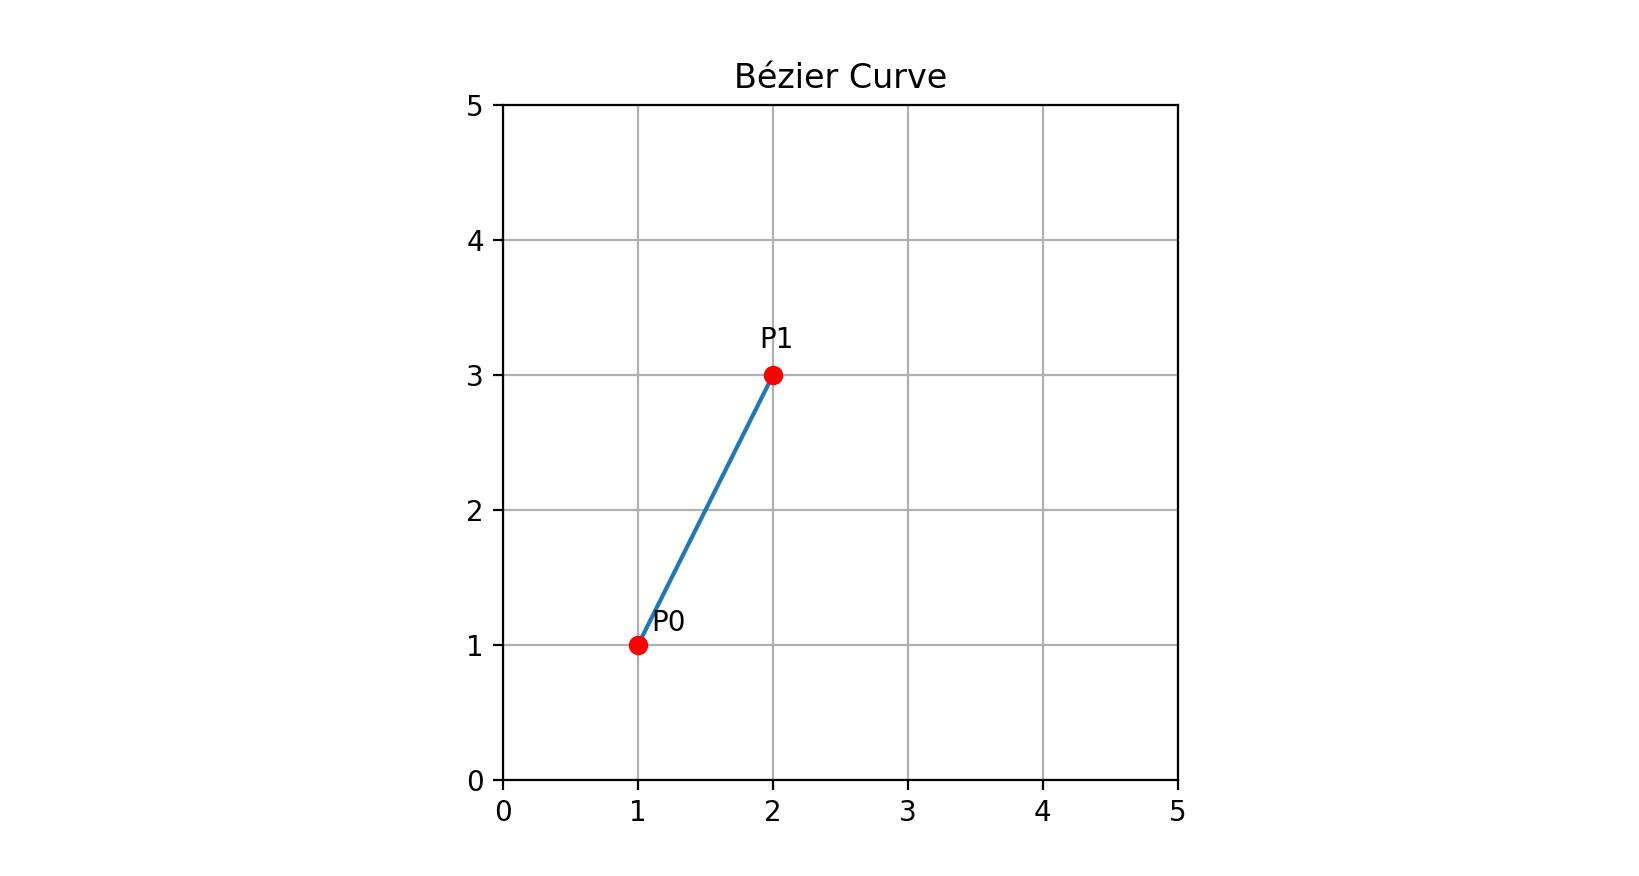
\includegraphics[width=15cm]{Figure_3}
    \centering
    \caption{Linear B\'ezier curve.}
    \label{fig:bez2}
\end{figure}

As $t$ increases from 0 to 1, the coordinates produced become further from $P_0$ and closer to $P_1$ because $P_0$ is getting subtracted away and $P_1$ is being added at equal rates. 

Drawing a simple line with a parametric equation is not particularly impressive. However, when the equation is rearranged to be a Bernstein polynomial, the formula can easily be adapted to accommodate more dimensions. Equation \ref{eq:bern1} is a 1\textsuperscript{st} order Bernstein polynomial with the control points as coefficients if rearranged like below.

\begin{equation}
    \label{eq:bern1}
    F(t) = (1-t)P_0 + t P_1
\end{equation}

Each term in the Bernstein polynomial is matched sequentially with a control point as a coefficient to create formulas for higher order polynomials (See Table \ref{tab:coeffs}).

\begin{table}[H]
    \centering
    \begin{tabular}{ | c | c c | c | }
        \hline
        $B_{n,i} (t)$ & Bernstein Term & CP Coefficient & Complete Term \\
        \hline
        $B_{1,0}$ & $1-t$ 		& $P_0$ & $(1-t)P_0$ 	    \\
        \hline
        $B_{1,1}$ & $t$ 		& $P_1$ & $tP_1$ 		    \\
        \hline
        $B_{2,0}$ & $(1-t)^2$ 	& $P_0$ & $(1-t)^2P_0$ 	    \\
        \hline
        $B_{2,1}$ & $2(1-t)t$ 	& $P_1$ & $2(1-t)tP_1$ 	    \\
        \hline
        $B_{2,2}$ & $t^2$ 		& $P_2$ & $t^2P_2$ 	        \\
        \hline
        $B_{3,0}$ & $(1-t)^3$ 	& $P_0$ & $(1-t)^3P_0$ 	    \\
        \hline
        $B_{3,1}$ & $3(1-t)^2t$ 	& $P_1$ & $3(1-t)^2P_1$	\\
        \hline
        $B_{3,2}$ & $3(1-t)t^2$ 	& $P_2$ & $3(1-t)t^2P_2$\\
        \hline
        $B_{3,3}$ & $t^3$ 		& $P_3$ & $t^3P_3$ 	        \\
        \hline
    \end{tabular}
    \caption{Bernstein polynomial, order 1 to 3, terms and corresponding B\'ezier control point coefficients.}
    \label{tab:coeffs}
\end{table}

For instance, below is a 2\textsuperscript{nd} order Bernstein polynomial, which uses 3 control points.

$$F(t)= (1-t)^2 P_0+2t(1-t) P_1+t^2 P_2$$

With 3 control points, the resulting graph forms a curve.

\begin{figure}[H]
    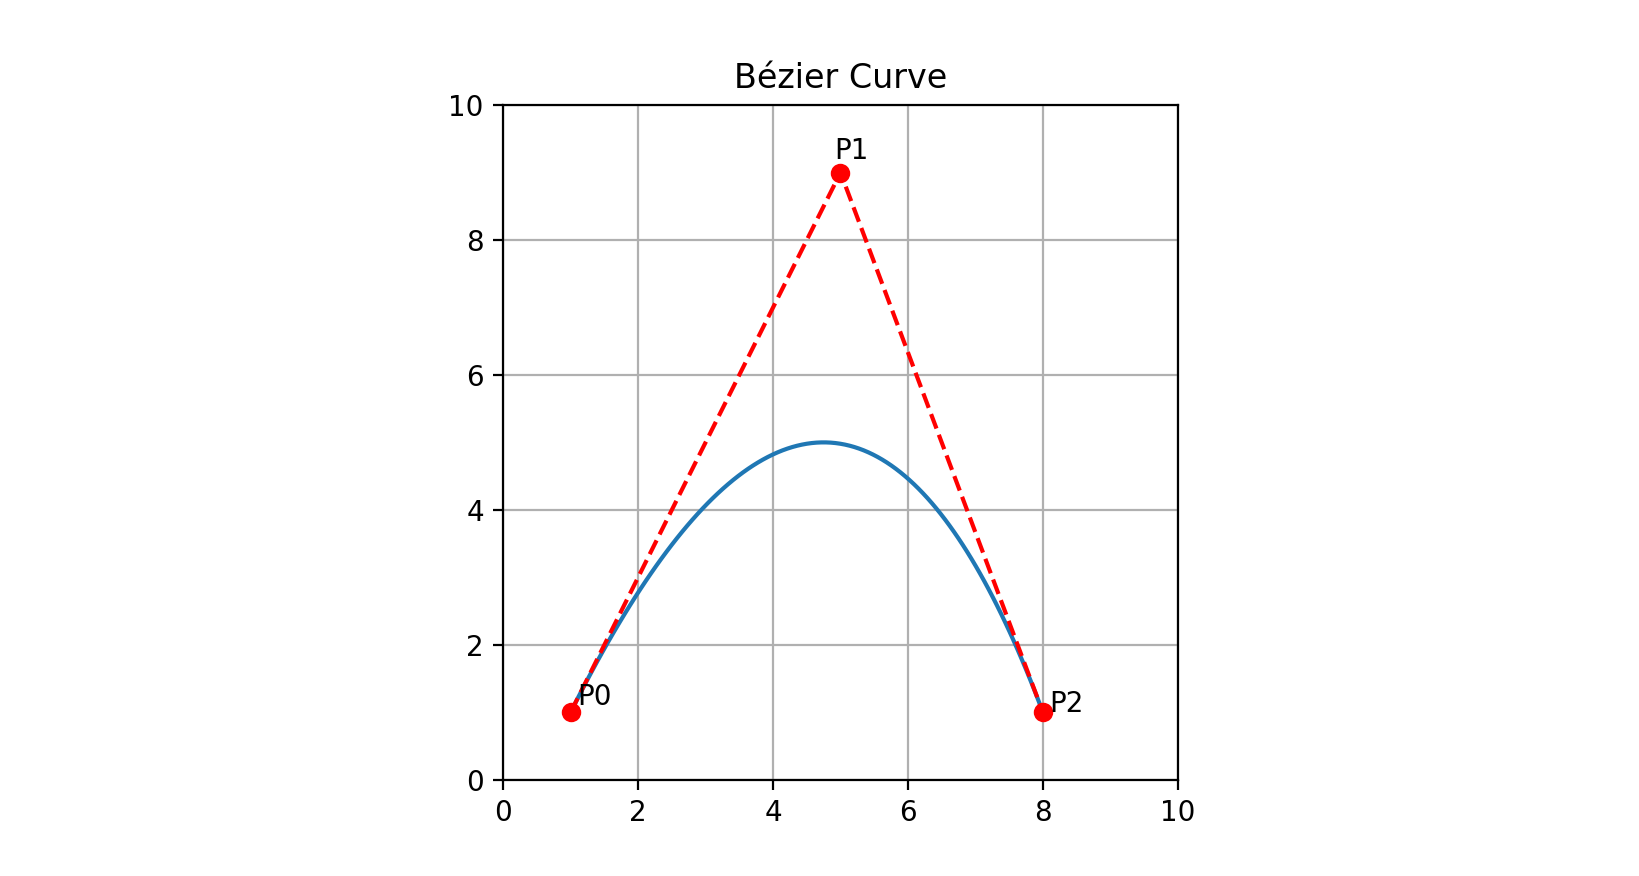
\includegraphics[width=15cm]{Figure_4}
    \centering
    \caption{B\'ezier curve with 3 control points, resulting from a 2\textsuperscript{nd} order Bernstein polynomial.}
    \label{fig:bez3}
\end{figure}

One byproduct of how the curve is formed is that the curve always lies completely within the area bounded by the control points. The curve in Figure \ref{fig:bez3} lies completely within the triangle formed by $P_0$, $P_1$, and $P_2$.

2\textsuperscript{nd} order Bernstein polynomial B\'ezier curves are referred to as quadratic B\'ezier curves. Another common form is the cubic B\'ezier curve, which uses a 3\textsuperscript{rd} order Bernstein polynomial.

$$F(t)=(1-t)^3 P_0+3t (1-t)^2 P_1+3t^2 (1-t) P_2+t^3 P_3$$

As can be expected, a 3\textsuperscript{rd} order polynomial has 4 terms and 4 control points.

\begin{figure}[H]
    \centering
    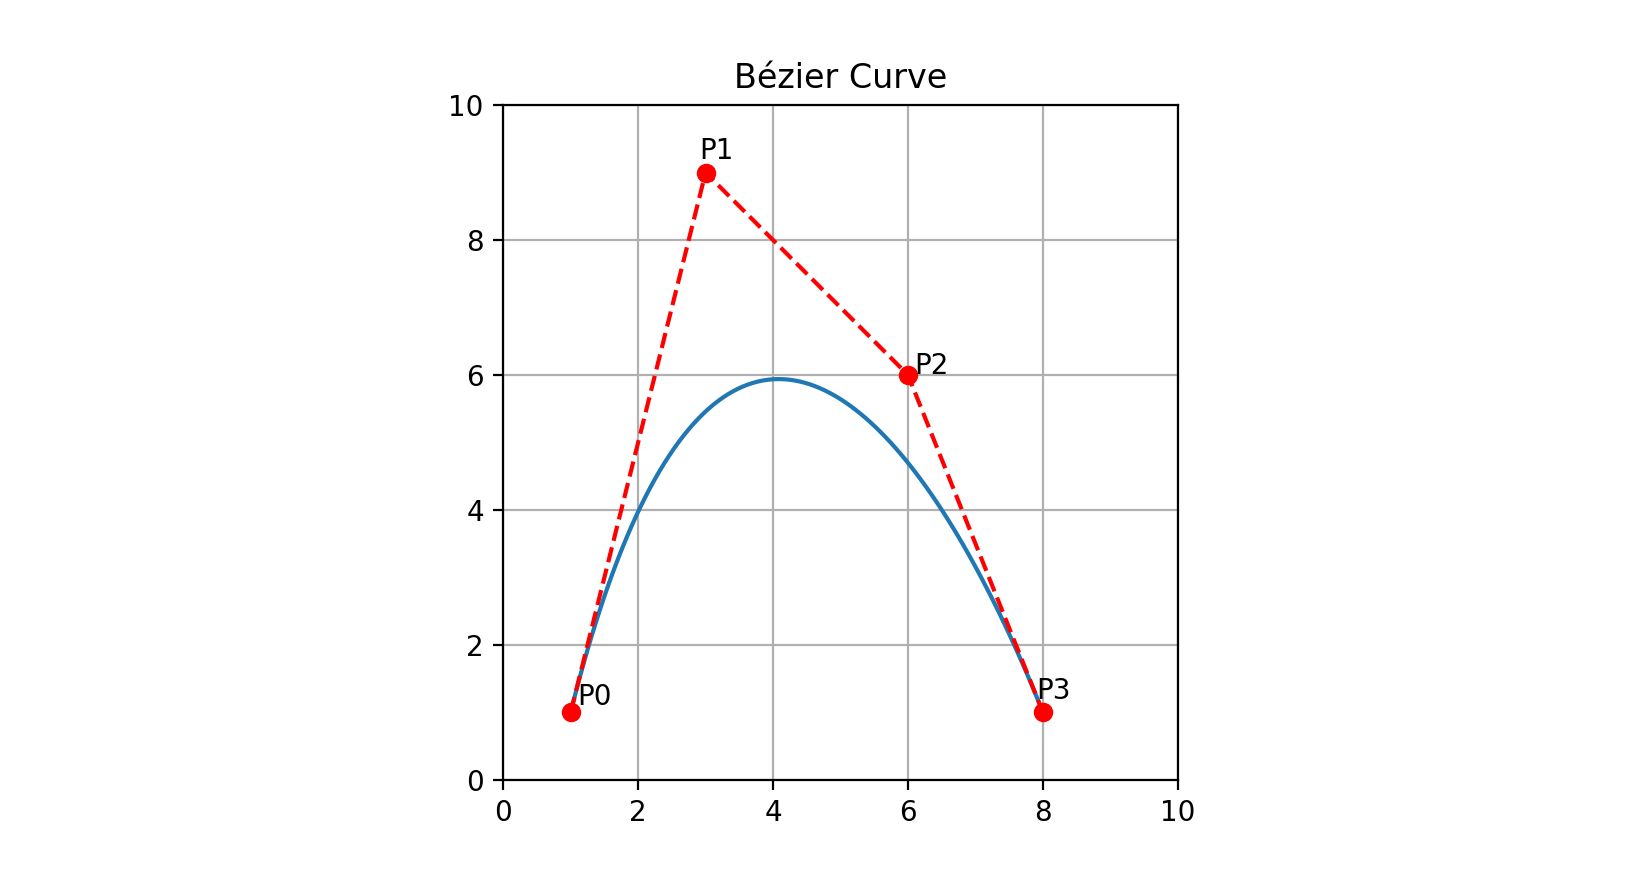
\includegraphics[width=15cm]{Figure_5}
    \caption{Cubic B\'ezier curve with 4 control points, generated with a 3\textsuperscript{rd} order Bernstein polynomial.}
    \label{fig:bez4}
\end{figure}

All of the B\'ezier graphs shown in this section (Figures \ref{fig:demo}, \ref{fig:demo2}, \ref{fig:bez2}, \ref{fig:bez3}, and \ref{fig:bez4}) were generated by the python script in Listing \ref{lst:bezier}.

A specific coordinate at any time $t$ can be solved for in one function with a summation of the Bernstein terms multiplied by their B\'ezier control point coefficient, as shown in Equation \ref{eq:decasteljau}. This formula is known as De Casteljau's algorithm, and is the formula used by computers as they render B\'ezier curves (Listing \ref{lst:bezier}).

\section{Applications}

\subsection{Fonts}

Until laser printers had a high enough dot density to produce legible text, digital fonts were virtually unnecessary and nonexistent. As printer technology developed, a digital typeface became a more and more likely development. B\'ezier curves ultimately answered the question of how to produce a digital text character with its easy to use and efficient to encode curves.

\begin{figure}[H]
    \centering
    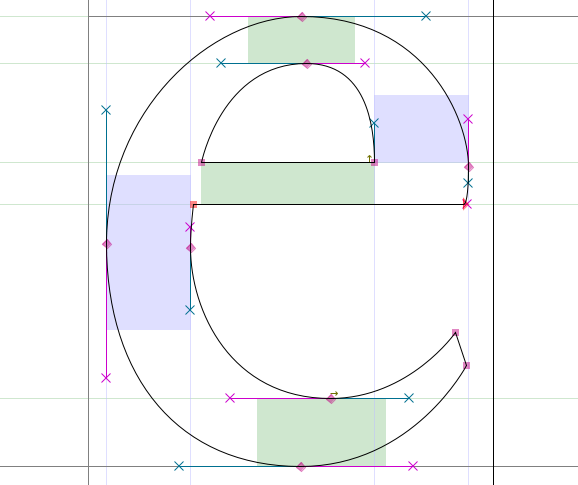
\includegraphics[width=10cm]{char}
    \caption{Letter `e' with visible B\'ezier control points \citep[9]{fontforge}}
\end{figure}

B\'ezier curves are suited well for fonts not only because computers can handle them well, but their adaptability and ease of adjustment lends toward the process of optical balancing. The design process of a font, even individual characters, requires very close attention to optical balance to make characters look and feel the way they are meant to be. Optimizing fonts is a topic for another discussion, so for now B\'ezier curves offer the flexibility needed to create quality fonts while also being efficient for computers to render. 

Computational efficiency is incredibly important for font rendering simply because text is rendered so frequently. As can be seen in the python code in Listing \ref{lst:bezier}, rendering a curve is a very simple task that only requires a few numerical arguments. As the primary method of displaying information in language form on a screen, text is rendered all the time. The efficiency of the B\'ezier curve allows text to not be a heavy burden on the CPU to render. 

The prevalence of B\'ezier curves in fonts has to do with the main digital font formats which are industry standards: TrueType and PostScript. PostScript was designed by Adobe in the early ‘80s as their core technology. It is a programming language dedicated toward document rendering. Fonts, as well as vector graphics, were drawn as a series of lines and cubic B\'ezier curves. These documents could be scaled to any resolution, and therefore were compatible with virtually any laser printer. 

Apple developed the TrueType outline font format to replace bitmap fonts in its Macintosh computers. TrueType was released with Macintosh System 7. It uses lines and quadratic B\'ezier curves. While quadratic curves are not as flexible as cubic curves with one less control point, they are computationally lighter for the same reason.

TrueType managed to become the dominant font standard after Apple licensed it to Microsoft. TrueType was added to the Windows operating system in 1991, and Microsoft published many TrueType fonts. Later on Microsoft created the OpenType format, which borrowed much of the underlying structure from TrueType, but included features for more control over typefaces. 

Both TrueType and PostScript replaced bitmap fonts entirely. Bitmap fonts were much harder to scale and less elegant than the curve-based successors. A bitmap font had to be recreated individually for each resolution, which was useful for making legibility adjustments at different sizes but was much more labor intensive to scale up or down for different sizes. Vector fonts could be automatically scaled, which is part of why they became the industry standard in digital typefaces. Now, on both Windows and macOS, TrueType, OpenType, and PostScript fonts are supported.


\subsection{Vectors}

PostScript’s use of cubic B\'ezier curves also made its way to the dominant vector graphic design software, Adobe Illustrator\textsuperscript{\textregistered{}}. Illustrator relies heavily on cubic B\'ezier curves to draw most every shape. The system is based entirely around the control points of the curves. The endpoints of curves are referred to as control points, while the two points that lie off the curve are called handles. The control point-based control scheme has been adopted as the default method of interaction universally in vector drawing software, and can be found in Illustrator and other popular vector programs such as CorelDRAW and Inkskape. 

\begin{figure}[H]
    \centering
    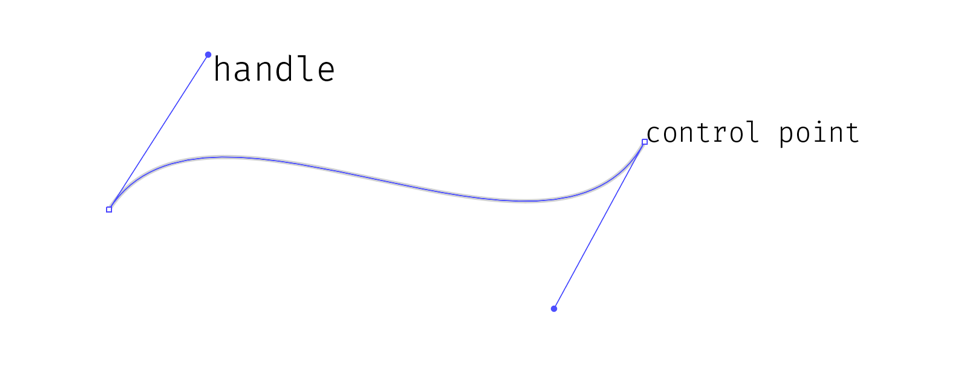
\includegraphics[width=\textwidth]{illustrator-ex}
    \caption{Example curve with control points visible, drawn the pen tool in Adobe Illustrator\textsuperscript{\textregistered{}}.}
\end{figure}

Vector design programs are a necessary tool for the creation of any digital graphic (websites, magazines, logos, brochures, advertisements, etc.). 

The Scalable Vector Graphics (SVG) file format is the common vector file format which can be read by mainstream vector software packages. It is written in eXtensible Markup Language (XML), a self-descriptive markup language meant to be legible for computers as well as humans. The SVG is an open standard format by the World Wide Web Consortium, used for graphics. SVGs are compatible with vector based graphic design programs, and can be integrated in-line with HTML. They are perfect for web use because the files are small, simple text files, but have the benefits of being infinitely scalable via the properties of vectors, hence the name Scalable Vector Graphic. For web use, this is ideal, since there are a wide range of screen resolutions to render web content on, and keeping large raster images on a web server can quickly become slow and cumbersome for a client that is loading the site. Of course, for a standard, vector based file, B\'ezier curves are the perfect way to take care of curves, shapes and fonts rendered in SVG files.

\section{Summary}
The intuitive nature of B\'ezier curves makes them perfect for artists and designers, but also the computational efficiency of Bernstein polynomials reduces load on the GPU of any machine that is rendering vector graphics. The perfect match of user and system benefits has resulted in widespread industry adoption in vector rendering and vector file formats. In today's climate of popular geometric and vector graphic design, as well as the ongoing and expanding use of print and digital text, B\'ezier curve technology is integral infrastructure for artists, designers, and readers around the world. 

\newpage
\bibliography{tynan-ee}
\bibliographystyle{apa}
\newpage

\section{Appendix}
\listoffigures
\listoftables

\newpage
\lstinputlisting[language=python, caption=B\'ezier Curve, label={lst:bezier}]{../py/bezier.py}
\lstinputlisting[language=python, caption=Bernstein Basis Functions, label={lst:bern}]{../py/bern.py}

\end{document}




